\section{Problem Definition}

\subsection{Limitations of Manual Software Testing}

A crucial aspect of software development is ensuring that the written code behaves as intended.  Today, this is particularly important, as software is playing an increasingly dominant role in our lives, from keeping our private data in the cloud to powering our ubiquitous smartphones.

Ideally, software would be written correctly by construction.  This was the way software engineering was envisioned to mature in the early days of computer science~\cite{dijkstra1976discipline}; the code would be written together with the mathematical proof of its correctness.

However, the decades of software development experience that followed have painted a different picture.  As it turns out, the software complexity---up to hundreds of millions of lines of code---and rapid pace of feature development have precluded a formal, rigorous approach.
%
With the exception of a few safety-critical segments, such as avionics~\cite{Astree}, automotive~\cite{automotive}, or medical equipment, most of the software industry today relies on \emph{testing} for its quality assurance~\cite{softwareMetrics}.

Testing a program consists of exercising multiple different paths through it and checking whether ``they do the right thing.''  In other words, testing is a way to produce partial evidence of correctness, and thus increase confidence in the tested software.  Yet, due to the typically poor coverage one can get today, testing often turns into a mere hunt for bugs.

In practice, most software test harnesses consist of manually written tests that are run periodically; regression test suites provide an automated way of checking whether new bugs have entered the code~\cite{codeComplete}.
%
Such suites tend to be tedious to write and maintain.  Statistics show that, on average, developers spend as much as half of their time doing testing~\cite{codeComplete}, and companies allocate up to a quarter of their IT budget for software testing~\cite{capgemini-world-quality}.

Despite the effort and resources invested, manual testing is prone to human error, and bugs eventually escape quality assurance and make it into production.  The problem is amplified by the security implications of having an increasing number of businesses online, and hence vulnerable to remote attacks.  Bugs are exploited to cause major disruptions, leaks of sensitive data, and the most prominent cases make headlines.

With a few exceptions---most notable being seL4~\cite{seL4}, a recent effort of formally verifying an operating system kernel---switching to a formal-driven development model is unfeasible for most of the software written today.
%
The second best option is to automate the software testing process itself.


\subsection{Automated Testing: Black-box Versus White-box}

The simplest (and most popular) form of automated testing consists of randomly generating program inputs and observing whether the program crashes~\cite{quickcheck}.  The inputs are typically obtained by fuzzing, i.e., randomly mutating a known valid input, such as an image file or a productivity suite document.
%
This form of testing is called ``blackbox'', because the input generation does not take into account the structure of the program under test~\cite{blackbox-testing}.
%
Despite their conceptual simplicity, fuzzers are effective at discovering bugs~\cite{afl,autodafe,skipfish} and are currently the state of practice in automated testing.

However, fuzzers are ineffective at discovering corner-case bugs---bugs that manifest only under particular inputs in the program.
%
For example, if a program checks whether its 32-bit integer input is the particular value 42, and only then it performs a null-pointer access, a random fuzzer has \emph{less than one in a billion} chance of hitting the bug with each input generated.
%
The vast majority of the generated inputs are therefore redundant.

This example hints at a better approach for test generation, which is to take the program structure into account when generating inputs.  This form of testing is called ``whitebox''; its goal is to generate inputs that take the program along previously unexplored execution paths.
%
Symbolic execution is the most successful automated whitebox testing technique to be applied on commodity software, which we discuss next in more detail.

\subsection{Systematic Path Exploration Using Symbolic Execution}

\begin{figure}
  \centering
  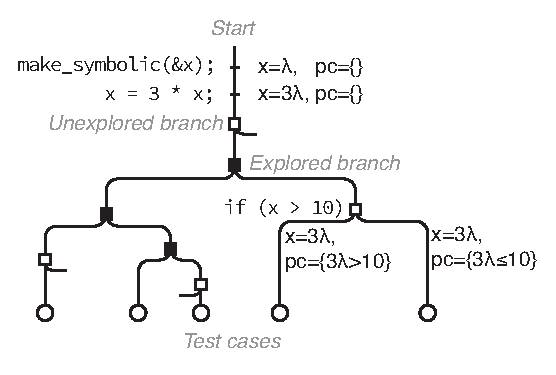
\includegraphics[width=3.5in]{figures/intro/symbex-tree}
  \caption{Symbolic execution tree for a simple example.  States maintain symbolic values for \codebit{x} and carry a path condition (pc).}
  \label{fig:intro:symbex-tree}
\end{figure}

Symbolic execution works by executing a program with \emph{symbolic} instead of concrete input values, to cover the entire input space and thus all possible program execution paths (Figure~\ref{fig:intro:symbex-tree}).  For instance, a function \codebit{foo(int x)} is executed with a symbolic variable $\lambda$ assigned to \codebit{x}.
%
Statements using \codebit{x} manipulate it symbolically: \codebit{x := x * 3} updates the value of \codebit{x} to $3 \cdot \lambda$.  During execution, the assignment of variables to expressions is kept in a \emph{symbolic store} of the program execution state.

Whenever symbolic execution encounters a conditional branch, the execution state forks into two states, whose executions proceed independently.  For each state, this process repeats for subsequent branches, turning an otherwise linear execution into a symbolic execution tree.

Each program state keeps the conjunction of the branch conditions taken on its path as a \emph{path condition}.
%
The path condition can be sent to a constraint solver to obtain a concrete assignment for the symbolic input (e.g., $\lambda = 42$), which takes the program along the exact execution path.  This input constitutes a \emph{test case} for the program.

The \emph{completeness}---systematic enumeration of all paths---and \emph{soundness}---each path is a real execution---of symbolic execution makes it highly effective at automatically generating high-coverage test suites, finding bugs, and even debugging.


% The satisfiability problem is NP-complete, which means there is no efficient (polynomial) algorithm available.  In practice, modern solvers can handle most formulas efficiently by using heuristics.  However, symbolic execution time is still dominated by constraint solving, as formulas can quickly become complex for non-trivial software.


%% The number of paths in the symbolic execution tree is roughly exponential in the number of program branches, with loops making the problem even worse.  As any non-trivial software can have at least thousands of branches, the size of the tree quickly becomes too large to be exhaustively covered in a reasonable amount of time.  This is called the ``path explosion'' problem.

Alas, symbolic execution is challenging to apply for non-trivial software.  The number of paths in the symbolic execution tree is roughly exponential in the number of program branches, with loops further amplifying the problem.  Even for moderately-sized programs with hundreds of branches, the size of the execution tree becomes too large to be completely covered in a reasonable amount of time.
%
This is commonly known as the ``path explosion'' problem and, in practice, symbolic execution engines resort to \emph{prioritizing} paths within a given time budget.


\subsection{The Environment Problem in Symbolic Execution}

For real-world software with thousands and even millions of lines of code, given the sheer size of the symbolic execution tree, mitigating path explosion alone is not sufficient.
%
For instance, consider a small system utility that prints at the terminal the contents of a file.  To perform this task, the program calls the operating system for accessing files and printing on the screen.
%
Symbolically executing this program potentially involves traversing tens of thousands of lines of kernel and library code, even if we're only interested in covering the code of the utility.

%% Instead, the symbolic execution engine should focus the execution on the system utility, and reduce the time spent in the environment, while keeping the behavior of the system at the program/environment interface as accurate as possible.

%% This is called the ``environment problem'' in symbolic execution and it is the distinctive scalability problem of symbolic execution for real-world software.  This is the topic of the thesis.

Instead, the symbolic execution engine should focus the exploration on the system utility, and reduce the time spent in its environment.
%
At the same time, the symbolic execution engine should provide to the program consistent data from the environment, in order to keep the execution sound and avoid missing feasible paths through the program.
%
This is called the ``environment problem'' in symbolic execution and it is the main scalability issue when applying symbolic execution on real-world software.

%% For example, one simple approach is to convert all the environment calls to concrete values.  This causes a single path per call through the environment, but this risks missing feasible paths in the utility itself.  For example, if opening a file with a symbolic name is both successful and failing, concretizing the file name will cause the program to experience only one behavior, say the successful one, and miss the error handling paths.

One possible approach for dealing with the environment problem is to simply let the calls into the environment go through concretely.  For instance, the symbolic parameters of a system call could be forcefully assigned concrete values before executing the system call.
%
However, this approach risks introducing inconsistencies in the execution and miss feasible paths in the target program itself.
%
For example, if opening a file with a symbolic name would either succeed or fail depending on the file name, concretizing to a valid file name would cause the symbolic execution to miss the error handling path in the program.

\newcommand{\cnineccolor}{\cellcolor{GreenYellow}}
\newcommand{\chefccolor}{\cellcolor{SkyBlue}}

\begin{table}
  \centering
  \small
  \begin{tabular}{r p{5cm} p{5cm}}
    \rule{0pt}{14pt} \textbf{Abstraction} & \cnineccolor Same-level & \chefccolor Nested \\
    \hline
    \bigskip Examples      & C program using a numerical library.    & Program written in a numerical computing language (e.g., Julia). \\
    
    \textbf{Encapsulation} & \chefccolor Loose & \cnineccolor Strong \\
    \hline
    \bigskip Examples      & Linux file system implemented as a kernel module.   & Linux file system implemented using the FUSE user-space interface. \\
    
    \textbf{Stability}   & \cnineccolor Stable    & \chefccolor Fast-changing \\
    \hline
        Examples          & A web application that uses a standard web interface, such as CGI.    & A web application that uses the fast-changing native API of its web server (e.g., Apache). \\
  \end{tabular}
  \caption{Examples of environment interfaces, classified along main design principles---abstraction and encapsulation---and stability in time.  Color overlays indicate design space coverage by \colorbox{GreenYellow}{\cnine} and \colorbox{SkyBlue}{\chef}.}
\end{table}


%%%%%%%%%%%%%%%%%%%%%%%%%%%%%%%%%%%%%%%%%%%%%%%%%%%%%%%%%%%%%%%%%%%%%%%%%%%%%%%%

\section{Solution Overview: A Tailored Approach to The Environment Problem}

Systematically addressing the environment problem is challenging, as its manifestations depend on the nature of the environment interface and its implementation.  This situation is best illustrated with examples.

For instance, a C program using a numerical library lies at the same abstraction level as the library, while a program performing the same operations, but written in a numerical computing language, e.g., Julia, is at a higher abstraction level than the language implementation.
%
A Linux file system implemented as a kernel module can interact with the entire kernel state, while the same file system code running in user-space through FUSE has a well-defined, encapsulated interface to the kernel.
%
Finally, the behavior of a web application using the fast-changing native API of its web server (e.g., Apache) would be more sensitive to the web server implementation changes than an equivalent application that uses a standard web interface, such as CGI.
%
In each of the three examples, a symbolic execution engine has one program to explore, yet it needs to approach the two alternative environments in fundamentally different ways.

%% This thesis addresses this problem by focusing on two points in the design space of the program/environment interface that collectively cover a wide range of real-world software: (1) low-level system software interacting with the operating system through the POSIX interface, and (2) high-level programs written in dynamic languages, such as Python, Ruby, or JavaScript.  These two points exhibit opposite characteristics.

This thesis addresses two instances of the environment problem, which collectively cover a wide range of real-world software: (1) system software interacting with the operating system, and (2) high-level programs written in dynamic languages, such as Python, Ruby, or JavaScript.
%
The two instances exhibit opposite characteristics.

%% On the one hand, the POSIX interface is properly encapsulated, well-documented, and stable.  Moreover, while the POSIX API consists of hundreds (or thousands?) of calls, its usage follows a power-law distribution [cite Radu's work], such that about 10s of them are commonly used in most software.

On the one hand, the operating system interfaces are typically stable and well-documented (e.g., POSIX).  Moreover, while they consist of hundreds of system calls, their usage follow a power-law distribution, such that most software only uses a small fraction of them.

%% On the other hand, the specifications of most popular dynamic languages are incomplete, vague, and change rapidly from one version of the language to another.

%% Moreover, these languages rely heavily on built-in methods, i.e. functions that are not implemented in the language itself, but execute as native C code in the interpreter.  This makes the program/environment interface highly porous, as the native calls can have arbitrary side effects on the program state.

On the other hand, the specifications of dynamic languages are incomplete and unstable.
%
Moreover, these languages rely heavily on built-in functions, i.e., functions that are not implemented in the language itself, but are C code part of the interpreter.  This makes the program/environment interface highly porous, as the built-in calls may have arbitrary side effects on the program state.

\subsection{Symbolic Models for a Stable Operating System Interface}

%% To address the first problem, we model much of the POSIX interface that we encountered when running widely used and complex real-world software, such as the Apache webserver, memcached, or the Python interpreter.

To address the environment problem for stable operating system interfaces, this thesis introduces \cnine, a symbolic execution platform with an accurate and efficient operating system model, as used by systems such as system utilities, web servers, or distributed systems.

%% Our insight is that, for the purpose of automated testing, the POSIX interface can be modeled efficiently on top of a few core abstractions: threads and processes, synchronization, and address spaces with shared memory.

%% On top of these abstractions, much of the POSIX interface can be implemented as guest code that substitutes the C standard library used by the target programs.

\cnine relies on the insight that, for the purpose of testing, the operating system interface can be modeled as guest code on top of a set of basic abstractions: threads and processes, synchronization, and address spaces with shared memory.
%
These abstractions need to be provided as primitives by the symbolic execution engine, while the rest of the model can be emulated as guest code, by substituting the standard C library used by the target programs.

%% We built the Cloud9 symbolic execution platform, which provides accurate and efficient models of POSIX abstractions such as files, network sockets, threads, processes, thread synchronization, IPC, signals, and other miscellaneous calls.

%% By using these symbolic models, Cloud9 is the first to efficiently target complex system utilities (e.g., curl), web servers, or distributed systems.

We prototyped \cnine for system code that uses the standard POSIX interface.  \cnine provides accurate and efficient models for files, network sockets, threads, processes, synchronization, IPC, signals, and other miscellaneous functions.
%
By using these models as substitutes for the complex kernel implementations, \cnine is the first to efficiently target complex system utilities such as \textsf{curl}, web servers such as Apache and lighttpd, or other networked services, such as memcached.


\subsection{Using Interpreters as Specifications for Fast-changing Languages}

%% The second problem lends itself to a different approach.  As the interface is volatile, porous, and complex, modeling it is an expensive ongoing engineering effort.

%% Instead, this thesis introduces the idea of using the interpreter as an ``executable language specification'': the interpreter runs in a lower-level (e.g., x86) symbolic execution engine while executing the target program.  The aggregate system acts as a high-level symbolic execution engine for the target program.

For incomplete and unstable dynamic language semantics, the environment problem lends itself to a different approach.
%
This thesis introduces the idea of using the interpreter as an ``executable language specification'': the interpreter runs in a lower-level (e.g., x86) symbolic execution engine, while it executes the target program.  In turn, the aggregate system acts as a high-level symbolic execution engine for the target program.

%% Mapping low-level interpreter paths to high-level program paths is done by segmenting the low-level paths into chunks corresponding to each high-level instruction executed.  Low-level paths with the same sequence of high-level instructions map to the same high-level path.

To map the low-level interpreter paths to high-level program paths, we partition the interpreter paths into chunks, one for each high-level instruction executed on the path. Then, the low-level paths with the same sequence of high-level instructions map to the same high-level path.

To circumvent the path explosion arising in the interpreter, we introduce Class-uniform Path Analysis (CUPA), a family of path prioritization heuristics for maximizing a given coverage metric.
%
CUPA works by grouping paths into equivalence classes, according to a coverage goal.  The prioritization is done by uniformly choosing groups instead of paths.  As a result, any path selection bias introduced by program locations with higher path explosion is contained within one equivalence class.

%% Additionally, we provide a set of fast recipes for eliminating common sources of path explosion in the interpreter.

%% We prototyped the Chef symbolic execution platform for interpreted languages and used it to obtain engines for Python, Lua, and JavaScript.

We prototyped these ideas in the \chef symbolic execution platform for interpreted languages.  With \chef, we obtained engines for Python and Lua, which generated test suites and found bugs in popular library packages.

%%%%%%%%%%%%%%%%%%%%%%%%%%%%%%%%%%%%%%%%%%%%%%%%%%%%%%%%%%%%%%%%%%%%%%%%%%%%%%%%

\section{Thesis Roadmap}

The rest of the thesis presents in detail the design, implementation, and evaluation of the two approaches to the environment problem.

Chapter~\ref{ch:relatedwork} provides more background on symbolic execution and the environment problem, by surveying the related work and positioning our contributions with respect to it.

Chapter~\ref{ch:cloud9} expands on the idea of modeling the operating system interface.  It presents the core abstractions that are built into the symbolic execution engine, then elaborates on the specifics of modeling the POSIX interface on top of them.

Chapter~\ref{ch:chef} presents the approach of using interpreters as executable language specifications.  It presents an overview of the Chef system, then it goes into the details of converting between the low-level symbolic execution of the interpreter and the high-level program execution.

Chapter~\ref{ch:evaluation} provides the experimental evaluation of the two systems we built, along two main dimensions: the effectiveness in generating test suites and finding bugs, and the scalability to real-world software.

Chapter~\ref{ch:paas} presents the ongoing work and longer-term vision of building a cloud-based testing service for cloud applications based on the techniques introduced in this thesis.

Chapter~\ref{ch:conclusion} ends the thesis with conclusions.

%%%%%%%%%%%%%%%%%%%%%%%%%%%%%%%%%%%%%%%%%%%%%%%%%%%%%%%%%%%%%%%%%%%%%%%%%%%%%%%%
%%%%%%%%%%%%%%%%%%%%%%%%%%%%%%%%%%%%%%%%%%%%%%%%%%%%%%%%%%%%%%%%%%%%%%%%%%%%%%%%









\iffalse
\section{Problem Definition}

\subsection{Limitations of Software Testing}

%% Software testing is resource-hungry, time-consuming, labor-intensive, and prone to human omission and error.  Despite massive investments in quality assurance, serious code defects are routinely discovered after software has been released~\cite{redHatSecurityX}, and fixing them at so late a stage carries substantial cost~\cite{codeComplete}.

Software testing is resource-hungry, time-consuming, labor-intensive, and prone to human omission and error.  A lot of bugs escape quality assurance into production, where they cause disruptions and data loss. For instance, in 2014, there were 19 CVE vulnerabilities reported on average per day, and estimates show that software bugs cost the global economy more than \$300 billion in 2013.

The security implications driven by today's connected world amplify the problem, with the largest disasters making the headlines.

At the same time, resources invested in testing are peaking. In 2014, about a quarter of the entire IT budget in enterprises was allocated to software testing, which was the highest figure to that date.  On average, developer teams spend as much as half of their time doing testing and fixing bugs.

Facing this situation, organizations recognize that software testing is cumbersome.  In a recent survey, more than two thirds of the organizations questioned admitted they have difficulties determining relevant tests for their software and pointed at the lack of adequate tools to support that.

\subsection{The Promise of Automated Test Case Generation}

%% Existing automated techniques, like model checking and symbolic execution, are highly effective at uncovering corner-case bugs typically missed by human scrutinity and hand-written tests.  However, their adoption in industrial general-purpose software testing has been hampered by two main challenges: applicability and scalability.

%% First, real-world systems interact heavily with the environment (e.g., through system calls or library calls) and may communicate with other parties (e.g., over sockets, IPC, shared memory).  A practical automated testing tool must be capable of handling these interactions while maintaining soundness (no false positives) and completeness (no false negatives).

%% Second, path explosion---the fact that the number of paths through a program is roughly exponential in program size---severely limits the extent to which large software can be thoroughly tested.

Existing automated techniques, like model checking and symbolic execution, are highly effective at uncovering corner-case bugs typically missed by human scrutinity and hand-written tests.

Symbolic execution, in particular, is attractive for targeting complex real-world software. It works by systematically enumerating all execution paths through a program.  It is attractive for three attributes: thoroughness (eventually enumerates all execution paths), soundness (unlike static analysis, there are no false positives), and flexibility (selection of paths can be prioritized, makes it attractive for targeting complex real-world software).

However, its adoption in industrial general-purpose software testing has been hampered by the path explosion problem---the fact that the number of paths through a program is roughly exponential in program size.

An important dimension of path explosion is the proliferation of execution paths outside the scope of the program of interest (e.g., inside system calls or library calls).  Dealing with that is challenging, as naively discarding possible executions may reduce the coverage, while abstracting (modeling) them inside the symbolic execution engine can be a significant engineering task.  We collectively call this set of challenges the \emph{environment problem} of symbolic execution.

In this thesis, we address the environment problem for two important classes of software that collectively cover a significant fraction of the real-world software running today: (1) low-level systems making rich use of the operating system interface, and (2) programs written in interpreted languages.  By expanding the scope of symbolic execution, we enable for the first time effective automated test case generation on a wide range of systems, which we demonstrate can find bugs and generate high-coverage test suites.

%%%%%%%%%%%%%%%%%%%%%%%%%%%%%%%%%%%%%%%%%%%%%%%%%%%%%%%%%%%%%%%%%%%%%%%%%%%%%%%%

\section{Background}

%% Testing a program consists of exercising many different paths through it and checking whether they ``do the right thing.''  In other words, testing is a way to produce partial evidence of correctness, and thus increase confidence in the tested software.  Yet, due to the typically poor coverage one can get today, testing often turns into a mere hunt for bugs.

%% In practice, most software test harnesses consist of manually written tests that are run periodically; regression test suites provide an automated way of checking whether new bugs have entered the code~\cite{codeComplete}.  Such suites tend to be tedious to write and maintain but, once in place, they can be reused and extended.  In practice, the state of the art consists mostly of fuzzing, i.e., trying various inputs in the hope of finding bugs and improving test coverage.

\subsection{Symbolic Execution Primer}

In research, the state of the art consists of model checkers and automated test generators based on symbolic execution~\cite{dart,klee}.  Instead of running a program with regular concrete inputs (e.g., $x\!=\!5$), symbolic execution consists of running a program with ``symbolic'' inputs that can take on all values allowed by the type (e.g., $x\!=\!\lambda$, where $\lambda \in \mathbb{N}$).  Whenever a conditional branch is encountered that involves a predicate $\pi$ that depends (directly or indirectly) on $x$, state and execution are forked into two alternatives: one following the then-branch ($\pi$) and another following the else-branch ($\neg \pi$). The two executions can now be pursued independently.  When a bug is found, test generators can compute concrete values for program inputs that take the program to the bug location.  This approach is efficient because it analyzes code for entire classes of inputs at a time, thus avoiding the redundancy inherent in fuzzing.

\subsection{Path Explosion}

%% The {\em first challenge} for such tools is path explosion, as mentioned earlier.  One way to cope is to memoize the symbolic execution of sub-paths into test summaries that can be subsequently reused when the same sub-path is encountered again, as done in compositional test generation~\cite{godefroid:compdyntest}.  Alternatively, it is possible to use various heuristics to prioritize the most interesting paths first, as done in \klee~\cite{klee}.  Another approach is to execute symbolically only paths that are of interest to the test, as done in selective symbolic execution~\cite{s2e}.

The size of the symbolic execution tree is exponential in the number of branches. Loops and recursion make things worse, with the number of paths potentially being infinite.

Dealing with the path explosion is crucial in ensuring the scalability of symbex.

Existing approaches work by either \emph{prioritizing}, \emph{folding}, or \emph{abstracting} paths.

Prioritizing paths means to use heuristics for determining the paths to select next, and optionally discarding the rest (pruning).  Randomness and static-analysis based heuristics are the most popular.

Folding paths means joining their representation either when they join in the CFG, or compositionally by computing summaries of sub-paths and reuse them when encountered again.

Abstracting paths mean replacing the execution of a complex part of the program with a simpler model that can be reasoned about symbolically more easily.

Neither of the approaches works well in all cases. The first two approaches help reduce the number of paths, at the expense of making each path more complex and slower (the entire complexity of the program is still encoded in the symbolic expressions).  The last approach simplifies the complexity, but in most cases it has a high upfront cost of determining the model, and risks being unsound (hence introducing false positives).

\subsection{The Environment Problem}

%% The {\em second challenge} is mediating between a program and its environment, i.e., symbolically executing a program that calls into libraries and the OS, or communicates with other systems, neither of which execute symbolically.  One possible approach is to simply allow the call to go through into the ``concrete'' environment (e.g., to write a file)~\cite{dart,exe}; unfortunately, this causes the environment to be altered for \emph{all} forked executions being explored in parallel, thus introducing inconsistency.  Another approach is to replace the real environment with a symbolic model, i.e., a piece of code linked with the target program that provides the illusion of interacting with a symbolically executing environment.  For instance, \klee uses a symbolic model of the file system~\cite{klee}. Of course, real-world programs typically interact in richer ways than just file I/O: they fork processes, synchronize threads, etc.  

%% We originally viewed the building of a complete environment model as an engineering task, but our ``mere engineering'' attempt failed: for any functionality that, in a normal execution, requires hardware support (such as enforcing isolation between address spaces), the core symbolic execution engine had to be modified.  The research challenge therefore is to find the minimal set of engine primitives required to support a rich model of a program's environment. 

Employing the three approaches is difficult when the source of path explosion is the program environment.  For instance, a program making use of libraries or OS syscalls.

One can employ pruning and allow the environment calls to go ``concretely'' in the environment.  In particular, the environment can be shared with the host, but this causes it to be altered for all forked executions and introduce inconsistency.

Another approach is to abstract the system (either model linked with program, or built into the engine).  But this is challenging for any non-trivial runtime, such as an operating system with hundreds of system calls.  For instance, \klee uses a symbolic model of the file system, but real-world programs interact in richer ways than just file I/O: they fork processes, synchronize threads, etc.

%%%%%%%%%%%%%%%%%%%%%%%%%%%%%%%%%%%%%%%%%%%%%%%%%%%%%%%%%%%%%%%%%%%%%%%%%%%%%%%%

\section{Solution Overview}

In this thesis, we address the path explosion of symbolic execution of real-world programs with complex environment interfaces by attacking two representative instances of the problem: low-level system software making rich use of the OS interface, and programs written in high-level interpreted languages, such as JavaScript, Python, Lua, etc.  These two correspond to two different environment scenarios: in the former, the interface is standardized and rather fixed, while in the latter it is highly volatile.

We prototyped the two approaches in two systems: Cloud9 is a symbolic execution platform for POSIX systems, while Chef is a platform for obtaining symbolic execution engines for interpreted languages by plugging the interpreter.

\subsection{Cloud9: Modeling Operating System Abstractions}

Cloud9 addresses the environment problem for the POSIX interface by leveraging the insight that only three abstractions need to be built into the engine, while the others can be implemented as guest code with less effort.  It also relies on the fact that in a symbolic environment, performance is less important (which in the real world would have been taken up by caches and additional layers of complexity).  By finding this sweetspot, Cloud9 keeps the model complexity low (hence reduced maintenance and extension effort), while supporting faithful execution for a wide set of real-world software, ranging from system utilities to web servers and distributed systems.

\subsection{Chef: Using Interpreters as Executable Language Specifications}

Chef addresses the environment problem for high-level interpreted languages (the environment here is the semantics and set of libraries available in the language).  The semantics of these languages are complex and volatile, so building a symbolic execution engine by hand is tedious.

Our insight is that we can use the interpreter of the language as an executable language specification.  By plugging in the interpreter into a low-level engine, we execute the high-level program.

We deal with the path explosion problem by providing a system where the high-level and low-level strategies are decoupled and can be optimized independently for the testing goal.

\subsection{Circumventing Path Explosion with CUPA}

Orthogonal to the two techniques addressing the environment problem, we further improved the performance of symbolic execution across all range of applications with two techniques.

Class Uniform Path Analysis is a path prioritization heuristic that leverages the observation that path explosion tends to be clustered in the so called ``fork bombs'':  regions of code, where states accumulate and bias a global selection strategy.  Instead, CUPA groups the states into classes, and then selects classes uniformly, effectively containing the path explosion.

\subsection{Addressing Path Explosion through Massive Parallelization}

%% We pursue a complementary approach---{\em parallel symbolic execution}---in which we symbolically execute a program in parallel on a cluster, thus harnessing the machines into a ``distributed computer'' whose aggregate CPU and memory surpass that of an individual machine.  An alternative to a cluster-based approach would be to run a classic single-node symbolic execution engine on a Blue Gene-like supercomputer with vast shared memory and CPUs communicating over MPI.  Supercomputers, however, are expensive, so we favor instead clusters of cheap commodity hardware.

%% One way to parallelize symbolic execution is by statically dividing up the task among nodes and having them run independently.   However, when running on large programs, this approach leads to high workload imbalance among nodes, making the entire cluster proceed at the pace of the slowest node~\cite{parallelSymbex}.  If this node gets stuck, for instance, while symbolically executing a loop, the testing process may never terminate.  Parallelizing symbolic execution on shared-nothing clusters in a way that scales well is difficult.

%% The work presented here aims to address these three challenges.  Cluster-based parallel symbolic execution (\S\ref{sec:parsymbex}) provides the illusion of running a classic symbolic execution engine on top of a large, powerful computer.  Without changing the exponential nature of the problem, parallel symbolic execution harnesses cluster resources to make it feasible to run automated testing on larger systems than what was possible until now. Our work complements and benefits all tools and approaches based on symbolic execution.  We describe a way to accurately model the environment (\S\ref{sec:posix}) with sufficient completeness to test complex, real software, like the Apache web server and the Python interpreter.  We present the APIs and primitives that we found necessary in developing a true testing platform (\S\ref{sec:platform}).  We show how using these APIs enables, for instance, finding errors in bug patches by reproducing environment conditions which otherwise would have been hard or impossible to set up with regular test cases.

Parallel symbolic execution.

\subsection{Symbolic Tests for Encapsulating the Symbolic Execution Task}

The {\em third challenge} is using an automated test generator in the context of a development organization's quality assurance processes.  To take full advantage of the automated exploration of paths, a testing tool must provide ways to control all aspects of the environment.  For example, there needs to be a clean API for injecting failures at the boundary between programs and their environment, there must be a way to control thread schedules, and so on.  There should be a way to programmatically orchestrate all environment-related events, but doing so should not require deep expertise in the technology behind the testing tools themselves.

\fi

%%% Local Variables: 
%%% mode: latex
%%% eval: (visual-line-mode)
%%% fill-column: 1000000
%%% TeX-master: "main"
%%% End:
